\section{Seeding by RF Noise} \label{Seed}

Seeding is important in RNG designs as it is fundamental to the randomness of PRNG. CC2538 suggests in its manual to  use the RF core to generate sample seed:(Section 16.2.2 in CC2538 User's Guide\cite{CC2538Manual})
\begin{quote}
For the CC2538, when a random value is required, writing the SOC\_ADC\_RNDL register with random bits from the IF\_ADC in the RF receive path seeds the LFSR.
\end{quote}
and also: (Section 23.12 in CC2538 User's Guide\cite{CC2538Manual})
\begin{quote}
Single random bits from either the I or Q channel can be read from the RFRND register.
\end{quote}

In case of Contiki, the driver only used the bits generated in I channel.

With respect to the randomness of this seeding method, the manual\cite{CC2538Manual} reported: (Section 23.12 in CC2538 User's Guide\cite{CC2538Manual})
\begin{quote}
Randomness tests show good results for this module. However, a slight DC component exists. In a simple test where the RFRND.IRND register was read a number of times and the data was grouped into bytes, about 20 million bytes were read. When interpreted as unsigned integers between 0 and 255, the mean value was 127.6518, which indicates that there is a DC component.
...
For the first 20 million individual bits, the probability of a 1 is $P(1) = 0.500602$ and $P(0) = 1 - P(1) = 0.499398$.
\end{quote}

Their test results are shown in \Cref{SeedResult}.

\begin{figure}[!t]
\centering
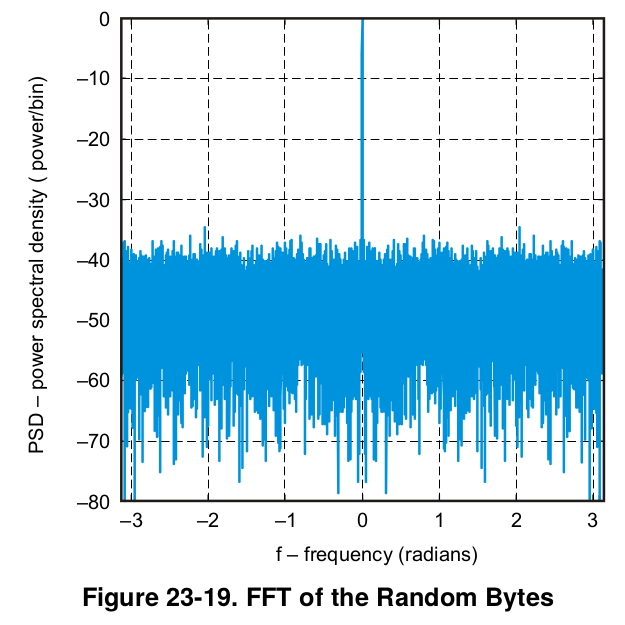
\includegraphics[width=2.5in]{fig/CC2538_Seed1.png}
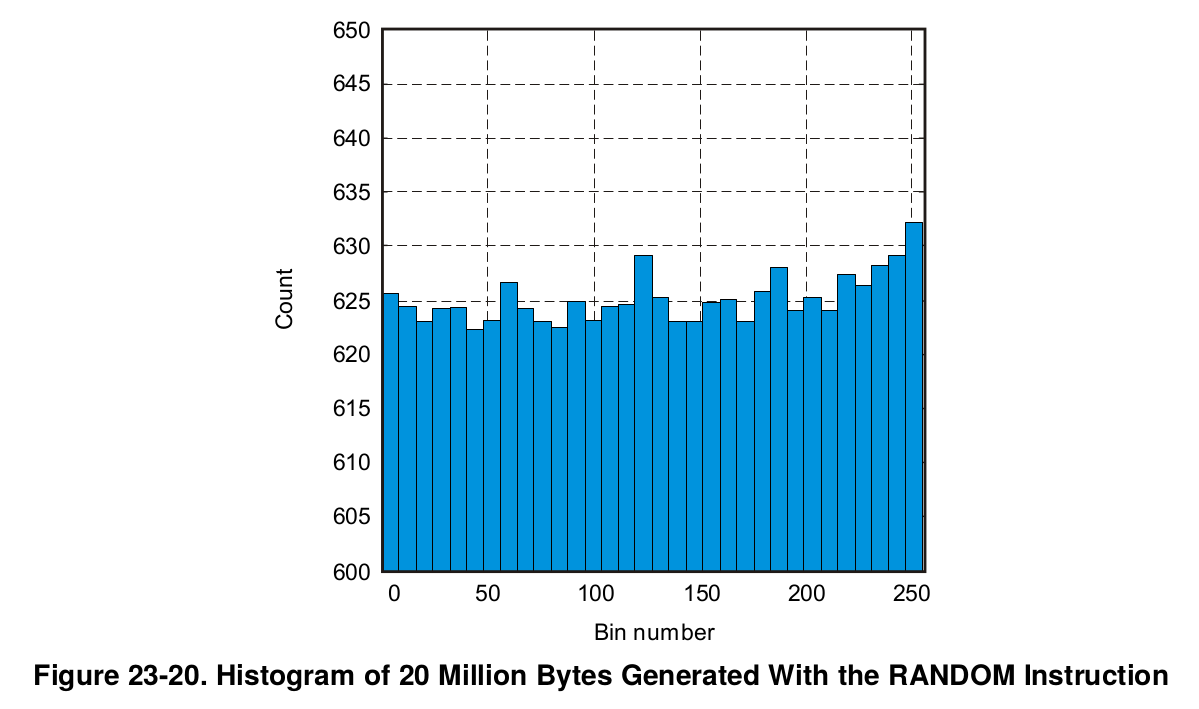
\includegraphics[width=2.5in]{fig/CC2538_Seed2.png}
\caption{RF core seeding result, from CC2538 User's Guide}
\label{SeedResult}
\end{figure}

To further verify the randomness of this seeding method, we applied the NIST Statistical Test Suite\cite{NISTTest} on 13263600 bits sampled by this seeding method using our application in \cite{prngtest}. Since each read to RFRND generates only $1$ bit, we concatenated all bits into one bit stream of length $13263600$. The bits has passed all tests in the NIST test suite, with $P(0) = 0.49995001$ and $P(1) = 0.50004999$. The full report and raw data are applicable at \cite{prngtest}.

%Despite the good randomness of the seed, sampling from RF noise remains sceptical from a security perspective as such physical source could be tampered remotely by sending jamming signal to the device.

The released documents did not explain further details of how IF\_ADC in the receive I/Q channels are translated to random bits. We have neither found any open document describes the RF design of CC2538. However, we noticed the same RNG design has been applied on several product in TI's SimpleLink series. Some of them provided better explanation of their RF core and RNG designs. 

In CC2430 user manual\cite{CC2430Manual}, we found a description of the RF core, shown in \Cref{CC2430RF}.

\begin{figure}[!t]
\centering
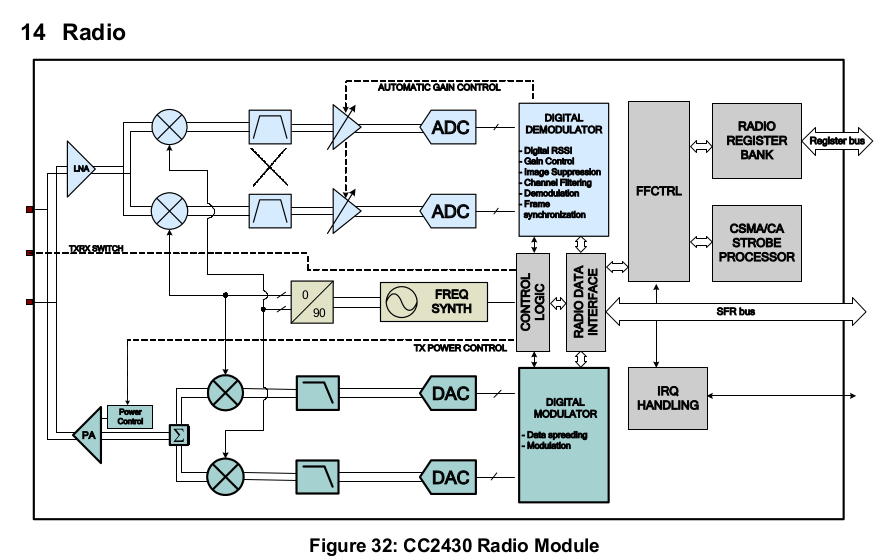
\includegraphics[width=2.5in]{fig/CC2430_Radio.png}
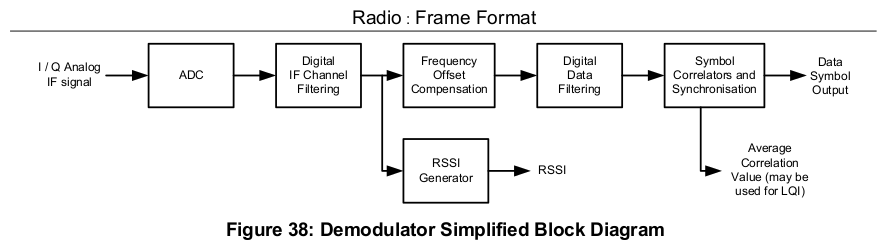
\includegraphics[width=2.5in]{fig/CC2430_Demodulator.png}
\caption{CC2430 RF Design, from CC2430 user manual\cite{CC2430Manual}}
\label{CC2430RF}
\end{figure}

\Cref{CC2430RF} explains that the input analogue signal to IF\_ADC has went through the following components:
\begin{itemize}
	\item Low Noise Amplifier (LNA) which amplifies the signal.
	\item Mixer which down converts the signal frequency. The Frequency Synthesiser is used as the local oscillator.
	\item Band pass filter which removes the out of band signals.
	\item The Automatic Gain Control (AGC) circuit further adjusts the signal strength to the input level of ADC.
\end{itemize}

CC2520 Data Sheet\cite{CC2520Manual} explains the random bit is actually the Least Significant Bit (LSB) from ADC: (Section 24 in \cite{CC2520Manual})
\begin{quote}
Single random bits from either the I or Q channel (configurable) can be output on GPIO pins at a rate of 8MHz. One can also select to xor the I and Q bits before they are output on a GPIO pin. These bits are taken from the least significant bit in the I and/or Q channel after the decimation filter in the demodulator.
\end{quote}

A block diagram is also provided, as shown in \Cref{CC2520RFRND}.
\begin{figure}[!t]
\centering
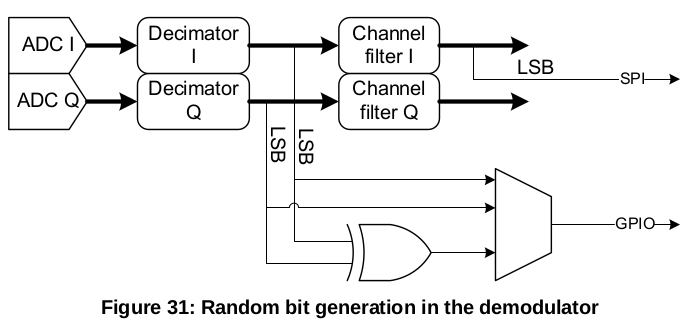
\includegraphics[width=2.5in]{fig/CC2520_RNG.png}
\caption{CC2520 RNG Design, from CC2520 user manual\cite{CC2520Manual}}
\label{CC2520RFRND}
\end{figure}

Interestingly, we noticed that CC2538, CC2520, CC253X and CC2540/41 reported exactly the identical randomness test result in their user manuals (\cite{CC2538Manual} \cite{ CC2520Manual} \cite{CC2530Manual}). We suspect the above evidences showed that CC2538 is very likely to have adopted the same design.

The design above would have explained the nice randomness of the seeding method. Denote $V_s$ as the analogue RF signal and $N$ as noise, the analogue input to the ADC, denote as  $V_{in}$, can be represented as:
\begin{equation} \label{V_in}
V_{in} = V_s + N
\end{equation}

The noise $N$ can be induced by multiple sources in practice, including:
\begin{itemize}
\item Noise produced by the signal source.
\item Environmental noise.
\item Noise induced by the components in the device itself.
\end{itemize}
%In practice, manipulating the noise could be difficult.

The random bit $b$ can be represented as:
\begin{equation} \label{RNDOutput}
b = LSB(V_{in}) = LSB(V_s + N)
\end{equation}
where $LSB() \in \{0,1\}$ represents the operation of taking the LSB of A/D conversion output.

Observing \Cref{RNDOutput}, one thing to be noticed is that any difference in $V_{in}$ larger than the scale of ADC, i.e. the voltage represented by its LSB, could flip $b$. According to CC2538 data sheet\cite{CC2538Datasheet}, the receiver can be sensitive to signals down to $-97dBm$ (typical value with $T_A = 25^{\circ}C$, $V_{DD} = 3V$ and $f_{C} = 2440MHz$). On the other hand, the typical environmental noise in our experimental environment is about $-92dBm$ which is significantly higher than the receiver sensitivity. We consider the result of the randomness test as an evidence to this sampling method.

\section{Biasing Seed by Radio Jamming}\label{Jamming}
 \Cref{RNDOutput} indicates that the random bit $b$ is jointly determined by the signal $V_s$ and noise $N$. Assuming the adversary can generate any signal, i.e. $V_s$ is fully  controlled by the adversary, manipulating $N$ turns out to be difficult in practice. For instance, noises accumulated by different amplification stages are physically inevitable. Hence predicted $V_{in}$ does not seem to be easily achievable in practice.

An alternative attempt is to provide the RF with illegal $V_{in}$. Two methods are considered in our experiments:
\begin{itemize}
	\item Saturation. This method attempts to provide the RF with a strong signal that is above its acceptance level.
	\item Decimation. This method attempts to provide the RF with a weak signal that is beneath its acceptance level.
\end{itemize}

Ideally we expect these illegal inputs will trigger the ADC into a fault state which could potentially result into a predictable output and thus predictable $b$. But in practice, decimation does not seem practical for the same reason that noises induced by the circuits themself are physically inevitable. This made saturation the only viable option.

Meanwhile, the undisclosed circuit design of the device also poses a great difficulty in our experiments. Without knowledge of the exact circuit design, it would be difficult to the deduce the most effective signal as well as to predict the outcome. Therefore we have only performed black box experiments. 

We used OpenMote\cite{OpenMote}, a CC2538 based SoC, for our experiments. The receiver has been configured to $2475MHz$ (channel 25 in 802.15.4) which is the default value for CC2538 in Contiki. 

We extended the length of each seed to 128 bits from RF in our experiments in coping to a potential PRNG design based on AES-128, although we still consider the bits are generated bitwise when applying the NIST test suite.

\subsection{Strong sine wave signal} \label{StrongSine}
The first signal we attempted was a strong sine wave signal. According to CC2538 data sheet\cite{CC2538Datasheet}, the saturation signal strength for the RF receiver is $10 dBm$. We have attempted to increase the input signal strength up to $13dBm$ which is roughly double of the saturation voltage but no bias was observed. The seed sampled under this signal has passed all tests in the NIST test suite.

The result implies that the AGC circuit could have tuned down the signal which might consequently prevented the seed from being biased. Although the exact AGC design for CC2538 is unclear, \Cref{AGC_QSL} demonstrates an example of AGC design using 4 Voltage Controlled Amplifiers (VGAs). The output signal is parallelly connected to a detector to estimate the signal strength. The output of detector is compared to a reference voltage and their difference is provided as a feedback to adjust the control voltage of VGAs. To prevent signal distortion caused by abrupt voltage change, such as during a lightning storm, many AGC design adopts an attack time before it adjusts the gain. \cite{AGC} provides a detailed description of different AGC designs. 

\begin{figure}[!t]
\centering
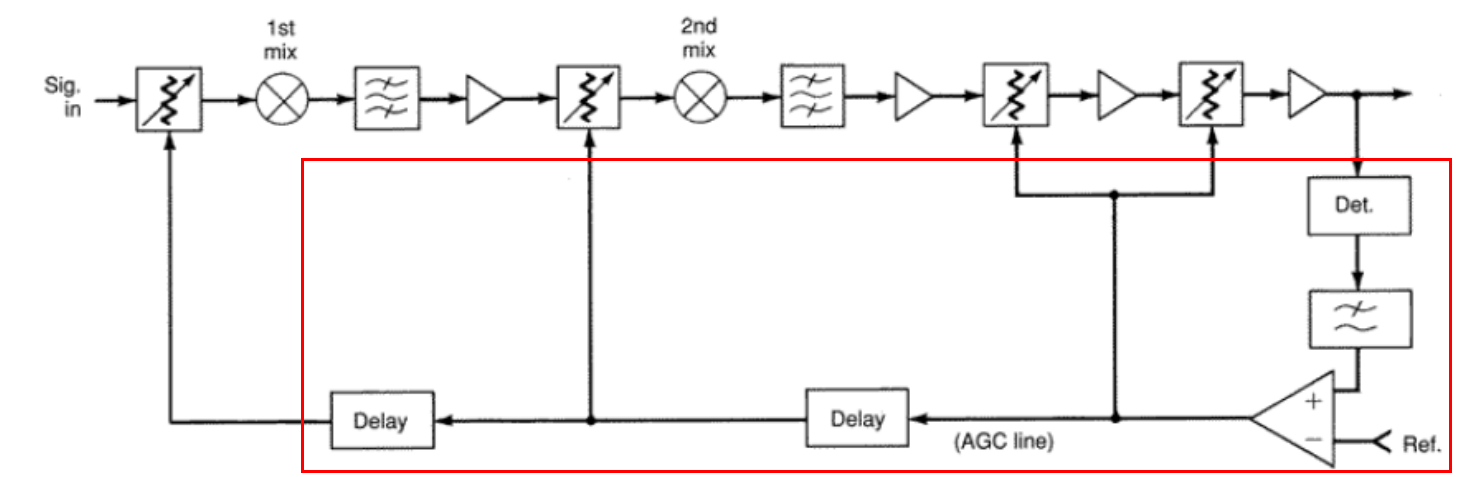
\includegraphics[width=2.5in]{fig/AGC.png}
\caption{Example of receiver AGC, from \cite{AGC_QSL}}
\label{AGC_QSL}
\end{figure}



%\subsection{Variable strength signal} \label{VariableStrength}
%Re-examining the experiments in \Cref{StrongSine} and the disclosed circuit designs, the AGC circuit could have tuned down the signal which might consequently prevented the seed from being biased. If this is the case, then the signal would need to get around the AGC to bias the seed.
%
%\begin{figure}[!t]
%\centering
%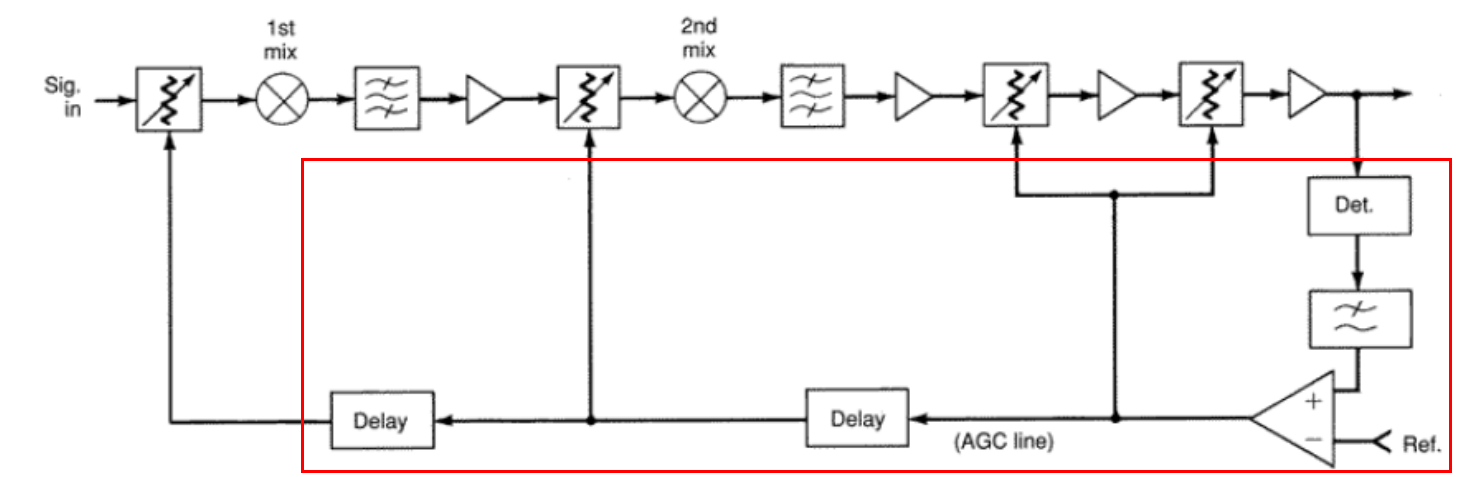
\includegraphics[width=2.5in]{fig/AGC.png}
%\caption{Example of receiver AGC, from \cite{AGC_QSL}}
%\label{AGC_QSL}
%\end{figure}
%
%Although the exact AGC design for CC2538 is unclear, \Cref{AGC_QSL} demonstrates an example of AGC design using 4 Voltage Controlled Amplifiers (VGAs). The output signal is parallelly connected to a detector to estimate the signal strength. The output of detector is compared to a reference voltage and their difference is provided as a feedback to adjust the control voltage of VGAs. To prevent signal distortion caused by abrupt voltage change, such as during a lightning storm, many AGC design adopts an attack time before it adjusts the gain. \cite{AGC} provides a detailed description of different AGC designs. 
% 
%The variable strength signal is therefore designed as an attempt to exploit the delay in AGC adjustments. To be more specifically, the signal is a sine wave at the working frequency which abruptly increases its strength to create a saturation, and then gradually decimates to tune down AGC. 
% 
%The signal can be achieved by multiplying a strong sine wave signal at the carrier frequency to a controlling sawtooth signal. The resulting signal would hopefully to:
%\begin{enumerate}
%	\item Be able to pass the band pass filter.
%	\item Generate bursts that saturates the ADC; therefore bits sampling during the transients will result into predicted bits.
%\end{enumerate}
%
%In our experiments, we used the default frequency $2475MHz$ for the carrier wave. The CC2538 User's Guide\cite{CC2538Manual} stated a programmable register (RFCORE\_XREG\_AGCCTRL3) which allows the user to select the AGC settle timing between 15, 20, 25 and 30 periods with default at 20. In the same document, the description of register RFCORE\_XREG\_RFC\_OBS\_CTRL0 stated that the random bit at both I and Q channels are updated at $8MHz$ which suggests that the receiver may have a sample rate of $16MHz$. Since the controlling signal should be slightly lower than the AGC adjustment frequency, this would give us a sawtooth signal near $0.8MHz$.
 
%Formally, denote the carrier signal $V_C$ as:
%\begin{equation}
%	V_{C}(t) = A\sin(\omega_{C} t)
%\end{equation}
%where $\omega_{C} = 2475MHz$ is the carrier frequency in our case. The signal needs to be strong enough to transiently saturate the ADC when the RF is detecting environmental noise. Assuming an 8 bit ADC and environmental noise at $-92dBm$, $V_{C}$ requires to be theoretically at least $-68dBm$.
%
%We control the amplitude by a sawtooth signal $V_{S}$ denote as:
%\begin{equation}
%	V_{S}(t) = - (\omega_S t \mod 1) + 1
%\end{equation}
%where $\omega_S$ is the frequency of bursts in the signal which is much lower than $\omega_C$ and should be slightly lower than the frequency of AGC adjustments.
%
%The desired signal is $V(t)$ is their product:
%\begin{equation}
%	V(t) = V_C(t)V_S(t)
%\end{equation}
%
%$V(t)$ is hopefully to have two properties:
%\begin{enumerate}
%	\item Being able to pass the band pass filter.
%	\item Generate bursts that saturates the ADC; therefore bits sampling during those period results into predicted bits.
%\end{enumerate}

%The signal source is implemented using Gnu Radio Companion\cite{GRC} with a HackRF One\cite{HackRFOne} directly connected to an OpenMote\cite{OpenMote}. However, no significant bias was reported by the NIST test suite. The exact cause of failure is unknown due to lack of design documentation but one potential reason might be that the period of transient is too short to significantly affect the seed.

\subsection{Strong constant signal} \label{Constant}
We then attempted a strong constant signal. The idea behind is to treat the whole circuit as a deterministic compression function that maps any $V_{in}$ to $\{0,1\}$. Under this assumption, the same $V_{in}$ should always generates the same $b$, either $0$ or $1$.

In order to achieve constant $V_{in}$ in \Cref{V_in}, the $V_s$ needs to be significantly greater than $N$ to suppress its impact in \Cref{RNDOutput}, as any ADC would have only a limited resolution.

For experimental purpose, we have configured three programmable LNAs in the AGC to their maximum gain ($6 + 21 + 9 = 36(dBm)$ in total) and has disabled the attenuator in Anti Aliasing Filter (AAF, up to $9dB$). We consider these modifications can be compensated by a strong signal amplifier in practice.

Gnu Radio Companion (GRC)\cite{GRC} and HackRF One\cite{HackRFOne} are used to implement the signal source. The corresponding GRC source file is applicable via \cite{prngtest}. \Cref{ConstantSignal} lists the parameters of the signal source configuration. The HackRF One is directly connected to the OpenMote antenna through a SMA cable to achieve the best signal strength.

\begin{table}[!t]
\caption{Signal source parameters for constant signal}
\label{ConstantSignal}
\centering
\begin{tabular}{|l|l|}
\hline
\textbf{Sample Rate} & 8 MHz             \\ \hline
\textbf{Output Type} & Complex           \\ \hline
\textbf{Waveform}    & Sine (can be any) \\ \hline
\textbf{Frequency}   & 2475 MHz          \\ \hline
\textbf{Amplitude}   & 0                 \\ \hline
\textbf{Offset}      & 10                \\ \hline
\end{tabular}
\end{table}

Applying the signal, we observed abnormally 0-runs, i.e. consecutive $0$ bits, appeared in the seeds as we increase IF gain to values above $10dB$. \Cref{IFvsP0} shows how $P(0)$ is biased and \Cref{IFvsN0} shows the maximum number of 0-runs in each seed. We can see that the bias has reached its peak at $IF\_gain = 22dB$ in both figures. At such gain $27.709\%$ of the 128 bit seeds have maximum 0-runs more than $64$ bits.

\begin{figure*}[!t]
\centering
\subfloat[$P(0)$ to IF Gain]{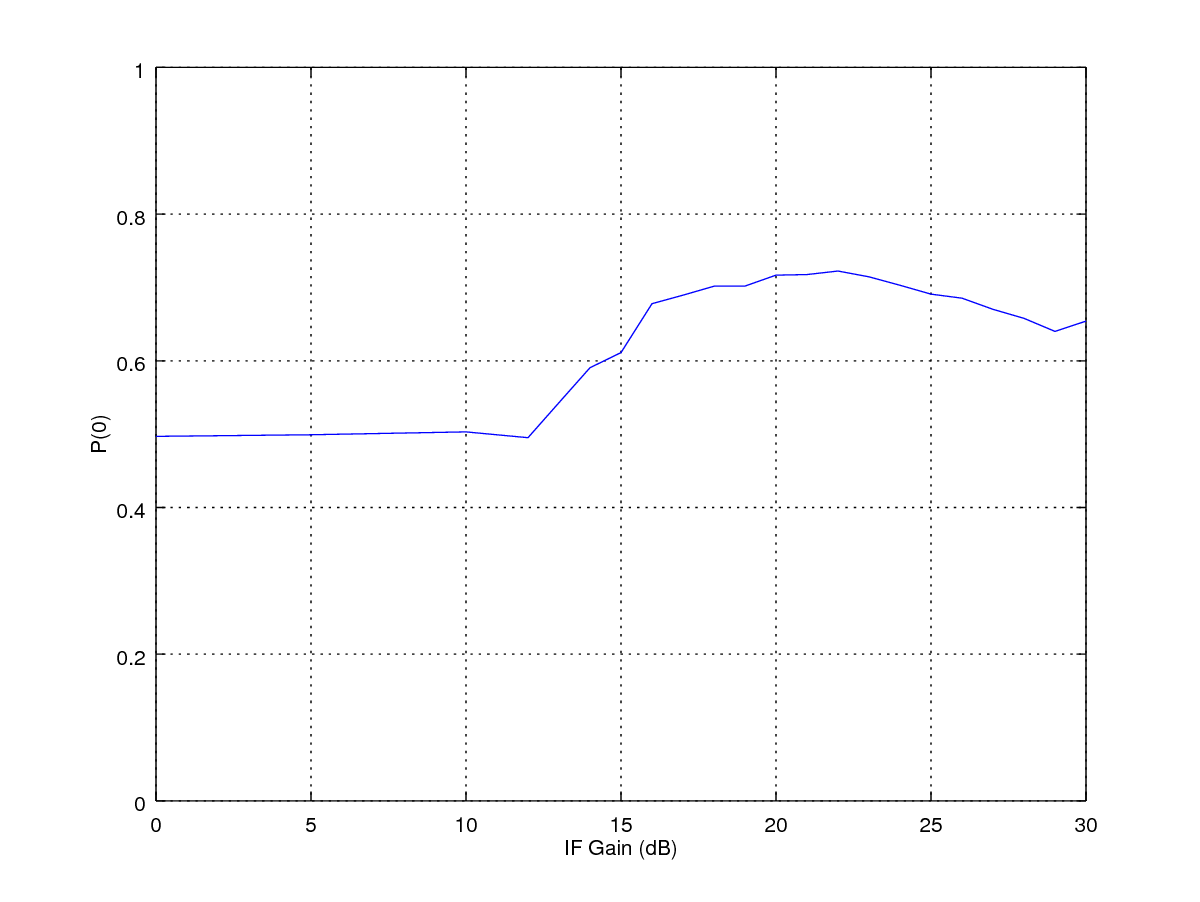
\includegraphics[width=2.5in]{fig/if_vs_P0_new.png}
\label{IFvsP0}}
\hfil
\subfloat[Average 0-runs to IF Gain]{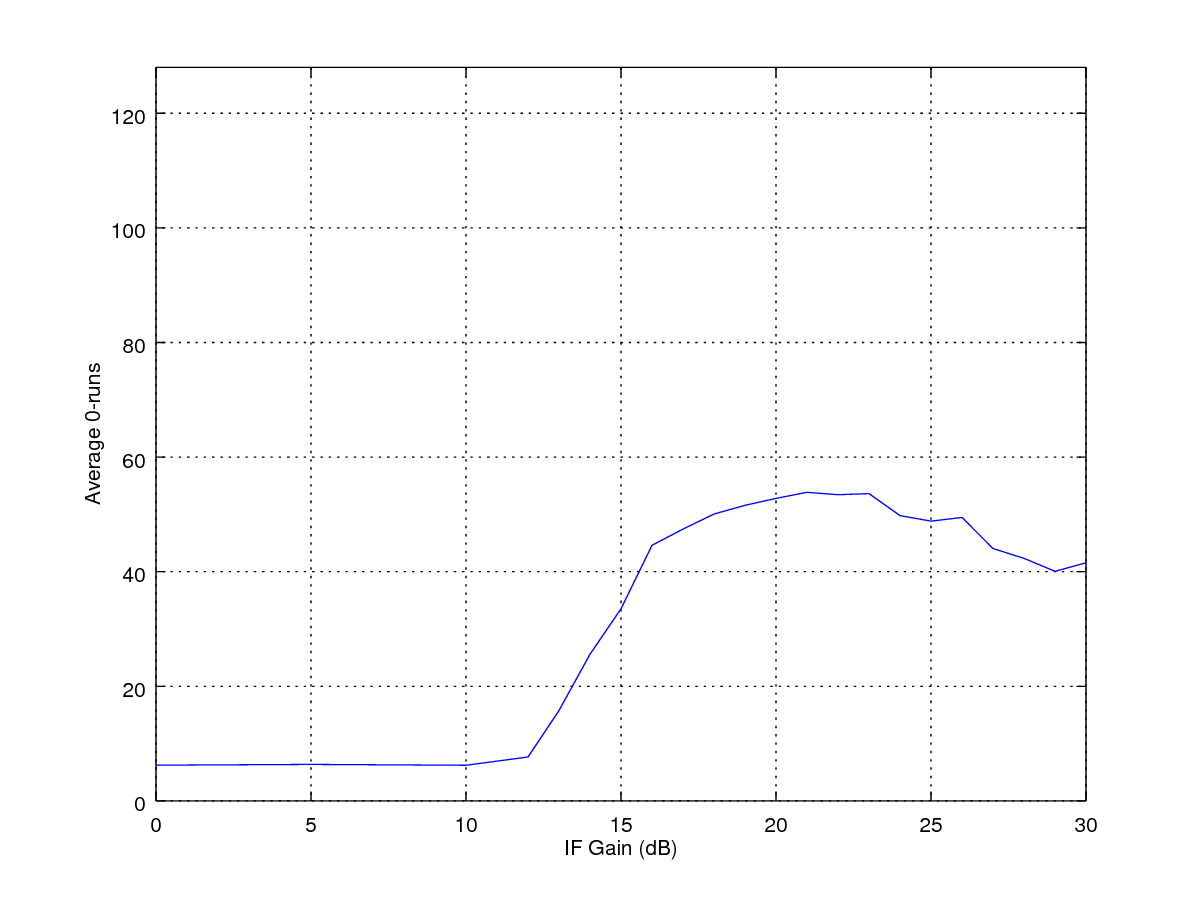
\includegraphics[width=2.5in]{fig/if_vs_N0_new.png}
\label{IFvsN0}}
\caption{Seed under Constant Signal}
\label{ConstantSignalBiased}
\end{figure*}

It is not surprise to see the sampled seeds have failed nearly all tests in the NIST test suite, indicating the seed has been strongly biased by our signal. A full report can be accessed at \cite{prngtest}.

We re-applied the signal to the same OpenMote we used for the previous experiments. A even stronger bias is observed as shown in \Cref{StronglyBiased}, with $17.820\%$ of the seeds ended in 128 consecutive $0$ bits.

We consider this may be caused by the strong sine wave signal in the previous experiments which permanent bias the device. We therefore restored its AGC configuration to default and re-ran the NIST test suite but the sampled seed has passed all tests as before. We also tested the device using example application provided by Contiki and found no malfunctioning on the device. The permanent bias does not seem to affect the device under normal operational status and can only be triggered by the constant signal. In practice, this indicates that such bias may be difficult to be notice for a victim.

\begin{figure*}[!t]
\centering
\subfloat[$P(0)$ to IF Gain]{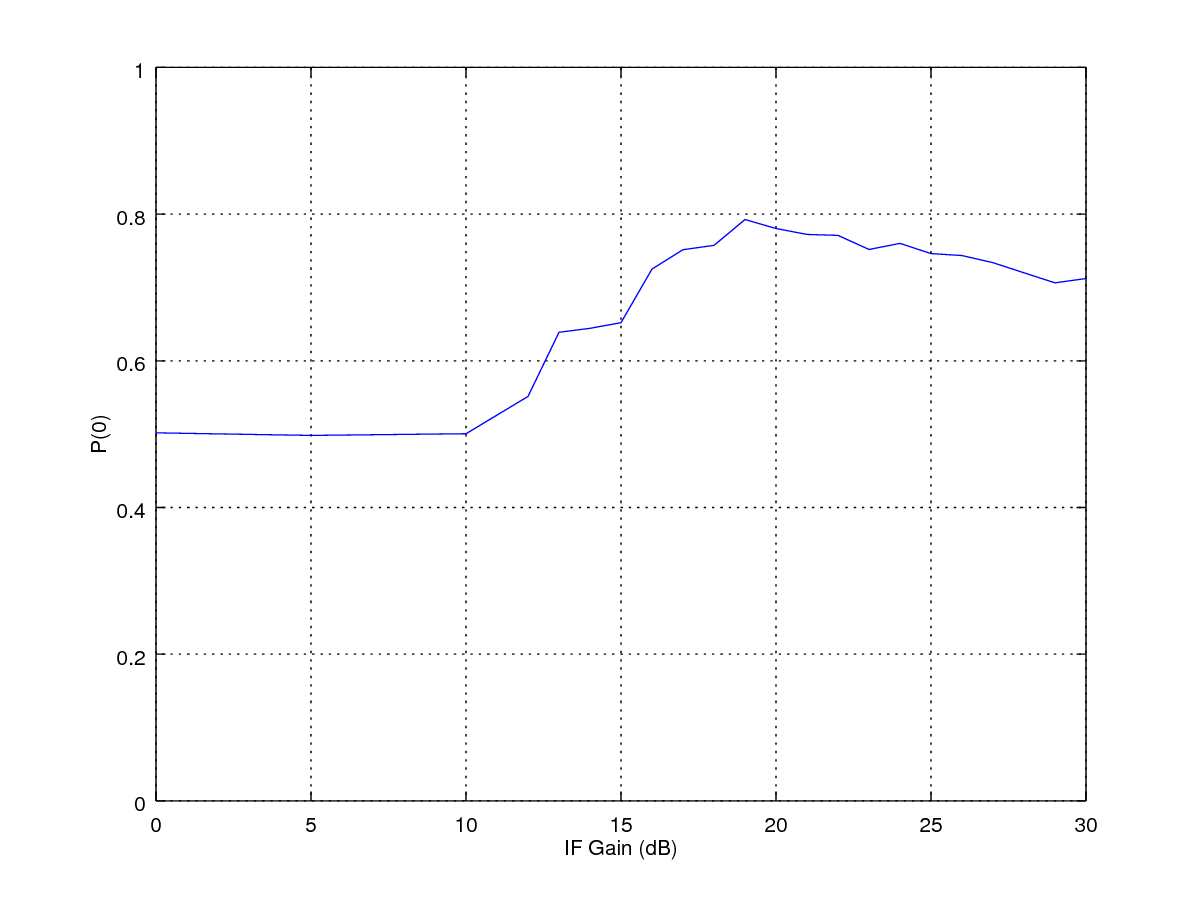
\includegraphics[width=2.5in]{fig/if_vs_P0.png}}
\hfil
\subfloat[Average 0-runs to IF Gain]{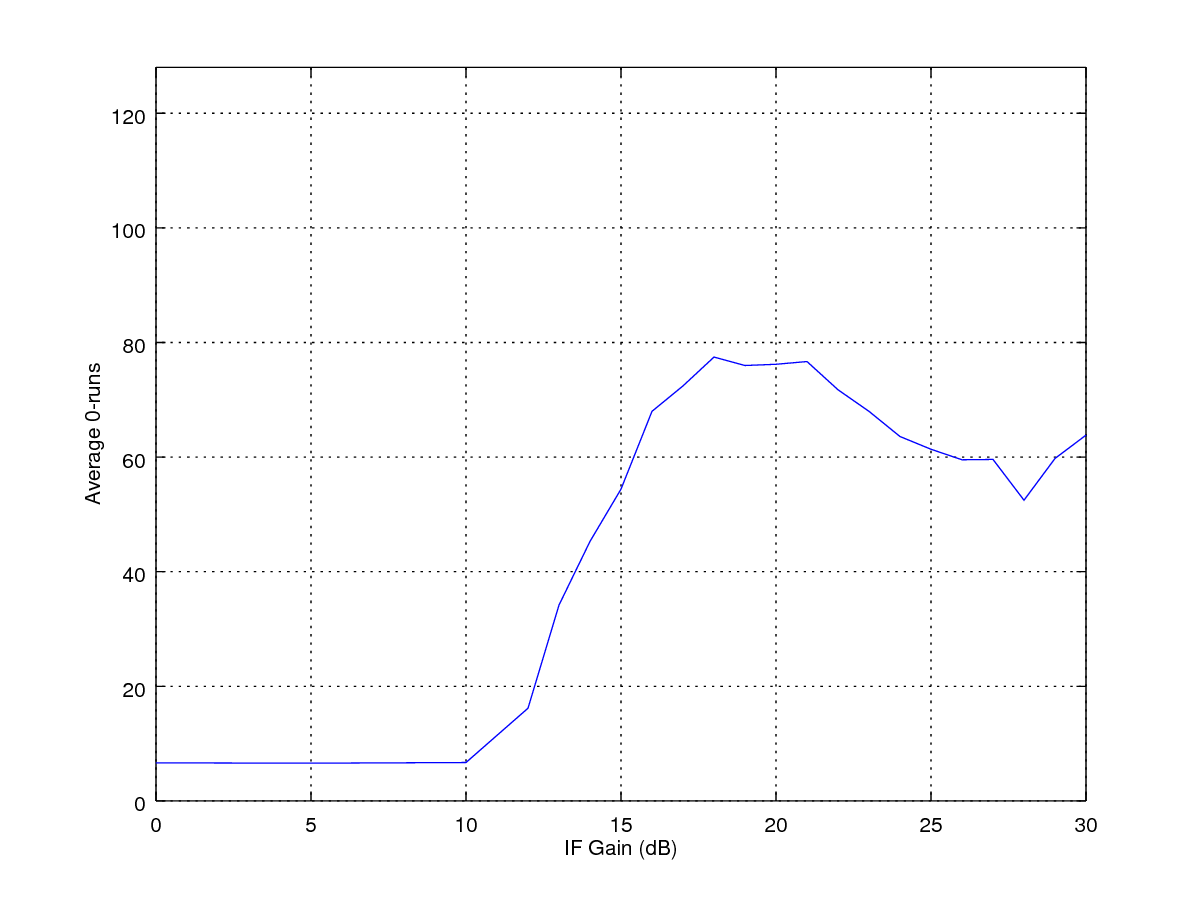
\includegraphics[width=2.5in]{fig/if_vs_N0.png}}
\caption{Biased Seed on OpenMote used in previous experiments}
\label{StronglyBiased}
\end{figure*}

Again due to lack of design documentation we can not explain how exactly the bias is triggered by the signal. Nevertheless our experiments have demonstrated that sampling seed using RF noise could potentially be biased by jamming signal and hence potentially breaching any cryptographic protocol relies on its randomness.